\documentclass[twoside]{book}

% Packages required by doxygen
\usepackage{fixltx2e}
\usepackage{calc}
\usepackage{doxygen}
\usepackage[export]{adjustbox} % also loads graphicx
\usepackage{graphicx}
\usepackage[utf8]{inputenc}
\usepackage{makeidx}
\usepackage{multicol}
\usepackage{multirow}
\PassOptionsToPackage{warn}{textcomp}
\usepackage{textcomp}
\usepackage[nointegrals]{wasysym}
\usepackage[table]{xcolor}

% Font selection
\usepackage[T1]{fontenc}
\usepackage[scaled=.90]{helvet}
\usepackage{courier}
\usepackage{amssymb}
\usepackage{sectsty}
\renewcommand{\familydefault}{\sfdefault}
\allsectionsfont{%
  \fontseries{bc}\selectfont%
  \color{darkgray}%
}
\renewcommand{\DoxyLabelFont}{%
  \fontseries{bc}\selectfont%
  \color{darkgray}%
}
\newcommand{\+}{\discretionary{\mbox{\scriptsize$\hookleftarrow$}}{}{}}

% Page & text layout
\usepackage{geometry}
\geometry{%
  a4paper,%
  top=2.5cm,%
  bottom=2.5cm,%
  left=2.5cm,%
  right=2.5cm%
}
\tolerance=750
\hfuzz=15pt
\hbadness=750
\setlength{\emergencystretch}{15pt}
\setlength{\parindent}{0cm}
\setlength{\parskip}{3ex plus 2ex minus 2ex}
\makeatletter
\renewcommand{\paragraph}{%
  \@startsection{paragraph}{4}{0ex}{-1.0ex}{1.0ex}{%
    \normalfont\normalsize\bfseries\SS@parafont%
  }%
}
\renewcommand{\subparagraph}{%
  \@startsection{subparagraph}{5}{0ex}{-1.0ex}{1.0ex}{%
    \normalfont\normalsize\bfseries\SS@subparafont%
  }%
}
\makeatother

% Headers & footers
\usepackage{fancyhdr}
\pagestyle{fancyplain}
\fancyhead[LE]{\fancyplain{}{\bfseries\thepage}}
\fancyhead[CE]{\fancyplain{}{}}
\fancyhead[RE]{\fancyplain{}{\bfseries\leftmark}}
\fancyhead[LO]{\fancyplain{}{\bfseries\rightmark}}
\fancyhead[CO]{\fancyplain{}{}}
\fancyhead[RO]{\fancyplain{}{\bfseries\thepage}}
\fancyfoot[LE]{\fancyplain{}{}}
\fancyfoot[CE]{\fancyplain{}{}}
\fancyfoot[RE]{\fancyplain{}{\bfseries\scriptsize Generated by Doxygen }}
\fancyfoot[LO]{\fancyplain{}{\bfseries\scriptsize Generated by Doxygen }}
\fancyfoot[CO]{\fancyplain{}{}}
\fancyfoot[RO]{\fancyplain{}{}}
\renewcommand{\footrulewidth}{0.4pt}
\renewcommand{\chaptermark}[1]{%
  \markboth{#1}{}%
}
\renewcommand{\sectionmark}[1]{%
  \markright{\thesection\ #1}%
}

% Indices & bibliography
\usepackage{natbib}
\usepackage[titles]{tocloft}
\setcounter{tocdepth}{3}
\setcounter{secnumdepth}{5}
\makeindex

% Hyperlinks (required, but should be loaded last)
\usepackage{ifpdf}
\ifpdf
  \usepackage[pdftex,pagebackref=true]{hyperref}
\else
  \usepackage[ps2pdf,pagebackref=true]{hyperref}
\fi
\hypersetup{%
  colorlinks=true,%
  linkcolor=blue,%
  citecolor=blue,%
  unicode%
}

% Custom commands
\newcommand{\clearemptydoublepage}{%
  \newpage{\pagestyle{empty}\cleardoublepage}%
}

\usepackage{caption}
\captionsetup{labelsep=space,justification=centering,font={bf},singlelinecheck=off,skip=4pt,position=top}

%===== C O N T E N T S =====

\begin{document}

% Titlepage & ToC
\hypersetup{pageanchor=false,
             bookmarksnumbered=true,
             pdfencoding=unicode
            }
\pagenumbering{alph}
\begin{titlepage}
\vspace*{7cm}
\begin{center}%
{\Large Pong \\[1ex]\large 1.\+0 }\\
\vspace*{1cm}
{\large Generated by Doxygen 1.8.13}\\
\end{center}
\end{titlepage}
\clearemptydoublepage
\pagenumbering{roman}
\tableofcontents
\clearemptydoublepage
\pagenumbering{arabic}
\hypersetup{pageanchor=true}

%--- Begin generated contents ---
\chapter{Pong Index Page Documentation}
\label{index}\hypertarget{index}{}\hypertarget{index_intro_sec}{}\section{Introduction}\label{index_intro_sec}
The project is a simple pong clone created in C++ using S\+F\+ML and Box2D. The project was created entirely by Daniel Thompson for De Montfort University, Student number P15230940.\hypertarget{index_running_sec}{}\section{Running The Game}\label{index_running_sec}
In order to run the game, launc Physics\+Game.\+exe located in the Debug folder.\hypertarget{index_controls_sec}{}\section{Controls}\label{index_controls_sec}
In order to start the game, press the space bar to spawn the pong ball. Once a player has scored, press space bar again to spawn another pong to continue. To exit the game, press the X button in the top right corner.\hypertarget{index_player1}{}\subsection{Player 1 Controls}\label{index_player1}
Player 1 is controlled as follows\+: Press the up arrow to move up, and the down arrow to move down.\hypertarget{index_player2}{}\subsection{Player 2 Controls}\label{index_player2}
Player 2 is controlled as follows\+: Press the W key to move up, and the S key to move down. 
\chapter{Hierarchical Index}
\section{Class Hierarchy}
This inheritance list is sorted roughly, but not completely, alphabetically\+:\begin{DoxyCompactList}
\item \contentsline{section}{game}{\pageref{classgame}}{}
\item \contentsline{section}{object}{\pageref{classobject}}{}
\begin{DoxyCompactList}
\item \contentsline{section}{paddle}{\pageref{classpaddle}}{}
\item \contentsline{section}{pong}{\pageref{classpong}}{}
\end{DoxyCompactList}
\end{DoxyCompactList}

\chapter{Class Index}
\section{Class List}
Here are the classes, structs, unions and interfaces with brief descriptions\+:\begin{DoxyCompactList}
\item\contentsline{section}{\hyperlink{classgame}{game} \\*Game class }{\pageref{classgame}}{}
\item\contentsline{section}{\hyperlink{classobject}{object} \\*Object class }{\pageref{classobject}}{}
\item\contentsline{section}{\hyperlink{classpaddle}{paddle} \\*Paddle class }{\pageref{classpaddle}}{}
\item\contentsline{section}{\hyperlink{classpong}{pong} \\*Pong class }{\pageref{classpong}}{}
\end{DoxyCompactList}

\chapter{File Index}
\section{File List}
Here is a list of all files with brief descriptions\+:\begin{DoxyCompactList}
\item\contentsline{section}{D\+:/\+Documents/\+Git\+Hub/\+Physics\+Game/include/\hyperlink{game_8cpp}{game.\+cpp} }{\pageref{game_8cpp}}{}
\item\contentsline{section}{D\+:/\+Documents/\+Git\+Hub/\+Physics\+Game/include/\hyperlink{game_8h}{game.\+h} }{\pageref{game_8h}}{}
\item\contentsline{section}{D\+:/\+Documents/\+Git\+Hub/\+Physics\+Game/include/\hyperlink{object_8cpp}{object.\+cpp} }{\pageref{object_8cpp}}{}
\item\contentsline{section}{D\+:/\+Documents/\+Git\+Hub/\+Physics\+Game/include/\hyperlink{object_8h}{object.\+h} }{\pageref{object_8h}}{}
\item\contentsline{section}{D\+:/\+Documents/\+Git\+Hub/\+Physics\+Game/include/\hyperlink{paddle_8cpp}{paddle.\+cpp} }{\pageref{paddle_8cpp}}{}
\item\contentsline{section}{D\+:/\+Documents/\+Git\+Hub/\+Physics\+Game/include/\hyperlink{paddle_8h}{paddle.\+h} }{\pageref{paddle_8h}}{}
\item\contentsline{section}{D\+:/\+Documents/\+Git\+Hub/\+Physics\+Game/include/\hyperlink{pong_8cpp}{pong.\+cpp} }{\pageref{pong_8cpp}}{}
\item\contentsline{section}{D\+:/\+Documents/\+Git\+Hub/\+Physics\+Game/include/\hyperlink{pong_8h}{pong.\+h} }{\pageref{pong_8h}}{}
\end{DoxyCompactList}

\chapter{Class Documentation}
\hypertarget{classgame}{}\section{game Class Reference}
\label{classgame}\index{game@{game}}


Game class.  




{\ttfamily \#include $<$game.\+h$>$}

\subsection*{Public Member Functions}
\begin{DoxyCompactItemize}
\item 
\hyperlink{classgame_a57f5809d56037158e9bafa65c8173609}{game} (b2\+World \&i\+World, int i\+Win\+Width, int i\+Win\+Height, double i\+S\+C\+A\+LE)
\begin{DoxyCompactList}\small\item\em Game controller constructor. \end{DoxyCompactList}\item 
\hyperlink{classgame_ae87abd20c4d8a7906fa48e690a5f1d07}{$\sim$game} ()
\begin{DoxyCompactList}\small\item\em Game controller destructor. \end{DoxyCompactList}\item 
virtual void \hyperlink{classgame_a7d9e3663af2341b48d6de562554f47b1}{draw} (sf\+::\+Render\+Window \&i\+Window)
\begin{DoxyCompactList}\small\item\em Draws all objects in the game. \end{DoxyCompactList}\item 
virtual void \hyperlink{classgame_aaac7fea645c92fd364bdccb24d59efd2}{update} (b2\+World \&i\+World)
\begin{DoxyCompactList}\small\item\em Updates all objects in the game. \end{DoxyCompactList}\item 
virtual void \hyperlink{classgame_a9733b814ab29dd4407441c17fa58b187}{handle\+Input} (b2\+World \&i\+World, sf\+::\+Event \&Event)
\begin{DoxyCompactList}\small\item\em Handles all input in the game. \end{DoxyCompactList}\item 
int \hyperlink{classgame_a5297f3ca1e18dfc8c4efd718b54b4982}{check\+Victory} ()
\begin{DoxyCompactList}\small\item\em Checks for player victory. \end{DoxyCompactList}\item 
void \hyperlink{classgame_a0b6f017a6d6d053ae89bc2ac3cbaa1aa}{center\+Text\+Pos} (sf\+::\+Text \&i\+Text, float i\+Actual\+Pos)
\begin{DoxyCompactList}\small\item\em Centers text. \end{DoxyCompactList}\item 
void \hyperlink{classgame_ae6f0753388b6ac52a3efd7073fc55934}{create\+Wall} (b2\+World \&i\+World, float X, float Y)
\begin{DoxyCompactList}\small\item\em Creates horizontal walls. \end{DoxyCompactList}\item 
void \hyperlink{classgame_a8d6319c1da22e9d41292feb3091bf562}{create\+Box} (b2\+World \&i\+World, int MouseX, int MouseY)
\begin{DoxyCompactList}\small\item\em Creates test boxes (Not used within game normally). \end{DoxyCompactList}\item 
\hyperlink{classpong}{pong} \hyperlink{classgame_a0f2725bdacb5162d7570a04cf8648490}{create\+Pong} (b2\+World \&i\+World)
\begin{DoxyCompactList}\small\item\em Creates Pong ball. \end{DoxyCompactList}\end{DoxyCompactItemize}


\subsection{Detailed Description}
Game class. 

Game class that holds all items within the pong game. Handles all events such as victory conditions, spawning pongs and spawning everything on run. Created by Daniel Thompson, P15230940. 

\subsection{Constructor \& Destructor Documentation}
\mbox{\Hypertarget{classgame_a57f5809d56037158e9bafa65c8173609}\label{classgame_a57f5809d56037158e9bafa65c8173609}} 
\index{game@{game}!game@{game}}
\index{game@{game}!game@{game}}
\subsubsection{\texorpdfstring{game()}{game()}}
{\footnotesize\ttfamily game\+::game (\begin{DoxyParamCaption}\item[{b2\+World \&}]{i\+World,  }\item[{int}]{i\+Win\+Width,  }\item[{int}]{i\+Win\+Height,  }\item[{double}]{i\+S\+C\+A\+LE }\end{DoxyParamCaption})}



Game controller constructor. 

\mbox{\Hypertarget{classgame_ae87abd20c4d8a7906fa48e690a5f1d07}\label{classgame_ae87abd20c4d8a7906fa48e690a5f1d07}} 
\index{game@{game}!````~game@{$\sim$game}}
\index{````~game@{$\sim$game}!game@{game}}
\subsubsection{\texorpdfstring{$\sim$game()}{~game()}}
{\footnotesize\ttfamily game\+::$\sim$game (\begin{DoxyParamCaption}{ }\end{DoxyParamCaption})}



Game controller destructor. 



\subsection{Member Function Documentation}
\mbox{\Hypertarget{classgame_a0b6f017a6d6d053ae89bc2ac3cbaa1aa}\label{classgame_a0b6f017a6d6d053ae89bc2ac3cbaa1aa}} 
\index{game@{game}!center\+Text\+Pos@{center\+Text\+Pos}}
\index{center\+Text\+Pos@{center\+Text\+Pos}!game@{game}}
\subsubsection{\texorpdfstring{center\+Text\+Pos()}{centerTextPos()}}
{\footnotesize\ttfamily void game\+::center\+Text\+Pos (\begin{DoxyParamCaption}\item[{sf\+::\+Text \&}]{i\+Text,  }\item[{float}]{i\+Actual\+Pos }\end{DoxyParamCaption})}



Centers text. 

\mbox{\Hypertarget{classgame_a5297f3ca1e18dfc8c4efd718b54b4982}\label{classgame_a5297f3ca1e18dfc8c4efd718b54b4982}} 
\index{game@{game}!check\+Victory@{check\+Victory}}
\index{check\+Victory@{check\+Victory}!game@{game}}
\subsubsection{\texorpdfstring{check\+Victory()}{checkVictory()}}
{\footnotesize\ttfamily int game\+::check\+Victory (\begin{DoxyParamCaption}{ }\end{DoxyParamCaption})}



Checks for player victory. 

\mbox{\Hypertarget{classgame_a8d6319c1da22e9d41292feb3091bf562}\label{classgame_a8d6319c1da22e9d41292feb3091bf562}} 
\index{game@{game}!create\+Box@{create\+Box}}
\index{create\+Box@{create\+Box}!game@{game}}
\subsubsection{\texorpdfstring{create\+Box()}{createBox()}}
{\footnotesize\ttfamily void game\+::create\+Box (\begin{DoxyParamCaption}\item[{b2\+World \&}]{i\+World,  }\item[{int}]{MouseX,  }\item[{int}]{MouseY }\end{DoxyParamCaption})}



Creates test boxes (Not used within game normally). 

\mbox{\Hypertarget{classgame_a0f2725bdacb5162d7570a04cf8648490}\label{classgame_a0f2725bdacb5162d7570a04cf8648490}} 
\index{game@{game}!create\+Pong@{create\+Pong}}
\index{create\+Pong@{create\+Pong}!game@{game}}
\subsubsection{\texorpdfstring{create\+Pong()}{createPong()}}
{\footnotesize\ttfamily \hyperlink{classpong}{pong} game\+::create\+Pong (\begin{DoxyParamCaption}\item[{b2\+World \&}]{i\+World }\end{DoxyParamCaption})}



Creates Pong ball. 

\mbox{\Hypertarget{classgame_ae6f0753388b6ac52a3efd7073fc55934}\label{classgame_ae6f0753388b6ac52a3efd7073fc55934}} 
\index{game@{game}!create\+Wall@{create\+Wall}}
\index{create\+Wall@{create\+Wall}!game@{game}}
\subsubsection{\texorpdfstring{create\+Wall()}{createWall()}}
{\footnotesize\ttfamily void game\+::create\+Wall (\begin{DoxyParamCaption}\item[{b2\+World \&}]{i\+World,  }\item[{float}]{X,  }\item[{float}]{Y }\end{DoxyParamCaption})}



Creates horizontal walls. 

\mbox{\Hypertarget{classgame_a7d9e3663af2341b48d6de562554f47b1}\label{classgame_a7d9e3663af2341b48d6de562554f47b1}} 
\index{game@{game}!draw@{draw}}
\index{draw@{draw}!game@{game}}
\subsubsection{\texorpdfstring{draw()}{draw()}}
{\footnotesize\ttfamily void game\+::draw (\begin{DoxyParamCaption}\item[{sf\+::\+Render\+Window \&}]{i\+Window }\end{DoxyParamCaption})\hspace{0.3cm}{\ttfamily [virtual]}}



Draws all objects in the game. 

\mbox{\Hypertarget{classgame_a9733b814ab29dd4407441c17fa58b187}\label{classgame_a9733b814ab29dd4407441c17fa58b187}} 
\index{game@{game}!handle\+Input@{handle\+Input}}
\index{handle\+Input@{handle\+Input}!game@{game}}
\subsubsection{\texorpdfstring{handle\+Input()}{handleInput()}}
{\footnotesize\ttfamily void game\+::handle\+Input (\begin{DoxyParamCaption}\item[{b2\+World \&}]{i\+World,  }\item[{sf\+::\+Event \&}]{Event }\end{DoxyParamCaption})\hspace{0.3cm}{\ttfamily [virtual]}}



Handles all input in the game. 

\mbox{\Hypertarget{classgame_aaac7fea645c92fd364bdccb24d59efd2}\label{classgame_aaac7fea645c92fd364bdccb24d59efd2}} 
\index{game@{game}!update@{update}}
\index{update@{update}!game@{game}}
\subsubsection{\texorpdfstring{update()}{update()}}
{\footnotesize\ttfamily void game\+::update (\begin{DoxyParamCaption}\item[{b2\+World \&}]{i\+World }\end{DoxyParamCaption})\hspace{0.3cm}{\ttfamily [virtual]}}



Updates all objects in the game. 



The documentation for this class was generated from the following files\+:\begin{DoxyCompactItemize}
\item 
D\+:/\+Documents/\+Git\+Hub/\+Physics\+Game/include/\hyperlink{game_8h}{game.\+h}\item 
D\+:/\+Documents/\+Git\+Hub/\+Physics\+Game/include/\hyperlink{game_8cpp}{game.\+cpp}\end{DoxyCompactItemize}

\hypertarget{classobject}{}\section{object Class Reference}
\label{classobject}\index{object@{object}}


Object class.  




{\ttfamily \#include $<$object.\+h$>$}

Inheritance diagram for object\+:\begin{figure}[H]
\begin{center}
\leavevmode
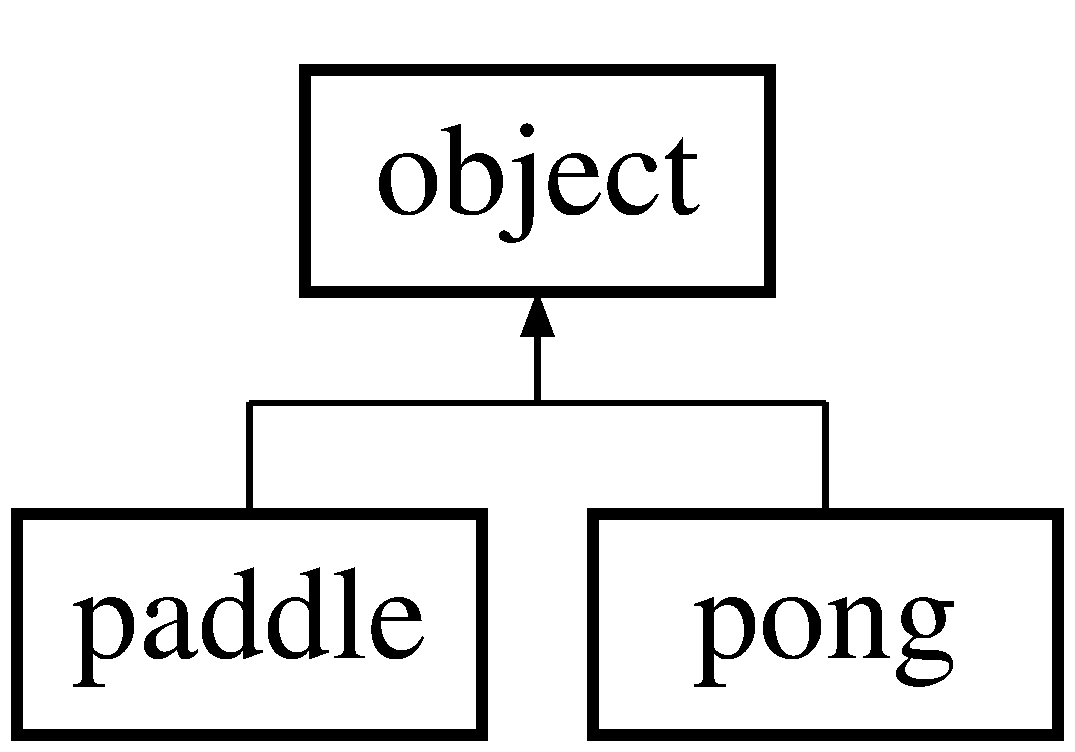
\includegraphics[height=2.000000cm]{classobject}
\end{center}
\end{figure}
\subsection*{Public Member Functions}
\begin{DoxyCompactItemize}
\item 
\hyperlink{classobject_a6444f1addfcba46e8a38e3a10afc5b55}{object} (b2\+World \&i\+World, float i\+X\+Pos, float i\+Y\+Pos, float i\+Width, float i\+Height, int i\+Restitution, double i\+S\+C\+A\+LE)
\begin{DoxyCompactList}\small\item\em Object constructor. \end{DoxyCompactList}\item 
b2\+Body $\ast$ \hyperlink{classobject_ae2e614e0e6af97805323193da7a1e7ff}{get\+Body} ()
\item 
b2\+Vec2 \hyperlink{classobject_a505665c0df5c44d5dfc77881fe5d95a4}{get\+Pos} ()
\begin{DoxyCompactList}\small\item\em Returns Box2D of object. \end{DoxyCompactList}\item 
void \hyperlink{classobject_a872e3c1ff75e786a58389852aad28a65}{set\+Dynamic} (bool Dynamic)
\begin{DoxyCompactList}\small\item\em Sets whether or not the Box2D body is dynamic. \end{DoxyCompactList}\item 
void \hyperlink{classobject_a74da589c4536cacfd76fa230a4dbee9e}{move} (b2\+Vec2 \&i\+Velocity)
\begin{DoxyCompactList}\small\item\em Sets the object\textquotesingle{}s velocity. \end{DoxyCompactList}\item 
void \hyperlink{classobject_a844b4128957b29e24370efe2d2cb3dca}{draw} (sf\+::\+Render\+Window \&window)
\begin{DoxyCompactList}\small\item\em Draws object on screen. \end{DoxyCompactList}\end{DoxyCompactItemize}


\subsection{Detailed Description}
Object class. 

Object class that contains basic structure of any physics object within the game. supports rendering and collision. Created by Daniel Thompson, P15230940. 

\subsection{Constructor \& Destructor Documentation}
\mbox{\Hypertarget{classobject_a6444f1addfcba46e8a38e3a10afc5b55}\label{classobject_a6444f1addfcba46e8a38e3a10afc5b55}} 
\index{object@{object}!object@{object}}
\index{object@{object}!object@{object}}
\subsubsection{\texorpdfstring{object()}{object()}}
{\footnotesize\ttfamily object\+::object (\begin{DoxyParamCaption}\item[{b2\+World \&}]{i\+World,  }\item[{float}]{i\+X\+Pos,  }\item[{float}]{i\+Y\+Pos,  }\item[{float}]{i\+Width,  }\item[{float}]{i\+Height,  }\item[{int}]{i\+Restitution,  }\item[{double}]{i\+S\+C\+A\+LE }\end{DoxyParamCaption})}



Object constructor. 



\subsection{Member Function Documentation}
\mbox{\Hypertarget{classobject_a844b4128957b29e24370efe2d2cb3dca}\label{classobject_a844b4128957b29e24370efe2d2cb3dca}} 
\index{object@{object}!draw@{draw}}
\index{draw@{draw}!object@{object}}
\subsubsection{\texorpdfstring{draw()}{draw()}}
{\footnotesize\ttfamily void object\+::draw (\begin{DoxyParamCaption}\item[{sf\+::\+Render\+Window \&}]{window }\end{DoxyParamCaption})}



Draws object on screen. 

\mbox{\Hypertarget{classobject_ae2e614e0e6af97805323193da7a1e7ff}\label{classobject_ae2e614e0e6af97805323193da7a1e7ff}} 
\index{object@{object}!get\+Body@{get\+Body}}
\index{get\+Body@{get\+Body}!object@{object}}
\subsubsection{\texorpdfstring{get\+Body()}{getBody()}}
{\footnotesize\ttfamily b2\+Body$\ast$ object\+::get\+Body (\begin{DoxyParamCaption}{ }\end{DoxyParamCaption})\hspace{0.3cm}{\ttfamily [inline]}}

\mbox{\Hypertarget{classobject_a505665c0df5c44d5dfc77881fe5d95a4}\label{classobject_a505665c0df5c44d5dfc77881fe5d95a4}} 
\index{object@{object}!get\+Pos@{get\+Pos}}
\index{get\+Pos@{get\+Pos}!object@{object}}
\subsubsection{\texorpdfstring{get\+Pos()}{getPos()}}
{\footnotesize\ttfamily b2\+Vec2 object\+::get\+Pos (\begin{DoxyParamCaption}{ }\end{DoxyParamCaption})}



Returns Box2D of object. 

Returns world position. \mbox{\Hypertarget{classobject_a74da589c4536cacfd76fa230a4dbee9e}\label{classobject_a74da589c4536cacfd76fa230a4dbee9e}} 
\index{object@{object}!move@{move}}
\index{move@{move}!object@{object}}
\subsubsection{\texorpdfstring{move()}{move()}}
{\footnotesize\ttfamily void object\+::move (\begin{DoxyParamCaption}\item[{b2\+Vec2 \&}]{i\+Velocity }\end{DoxyParamCaption})}



Sets the object\textquotesingle{}s velocity. 

\mbox{\Hypertarget{classobject_a872e3c1ff75e786a58389852aad28a65}\label{classobject_a872e3c1ff75e786a58389852aad28a65}} 
\index{object@{object}!set\+Dynamic@{set\+Dynamic}}
\index{set\+Dynamic@{set\+Dynamic}!object@{object}}
\subsubsection{\texorpdfstring{set\+Dynamic()}{setDynamic()}}
{\footnotesize\ttfamily void object\+::set\+Dynamic (\begin{DoxyParamCaption}\item[{bool}]{Dynamic }\end{DoxyParamCaption})}



Sets whether or not the Box2D body is dynamic. 



The documentation for this class was generated from the following files\+:\begin{DoxyCompactItemize}
\item 
D\+:/\+Documents/\+Git\+Hub/\+Physics\+Game/include/\hyperlink{object_8h}{object.\+h}\item 
D\+:/\+Documents/\+Git\+Hub/\+Physics\+Game/include/\hyperlink{object_8cpp}{object.\+cpp}\end{DoxyCompactItemize}

\hypertarget{classpaddle}{}\section{paddle Class Reference}
\label{classpaddle}\index{paddle@{paddle}}


Paddle class.  




{\ttfamily \#include $<$paddle.\+h$>$}

Inheritance diagram for paddle\+:\begin{figure}[H]
\begin{center}
\leavevmode
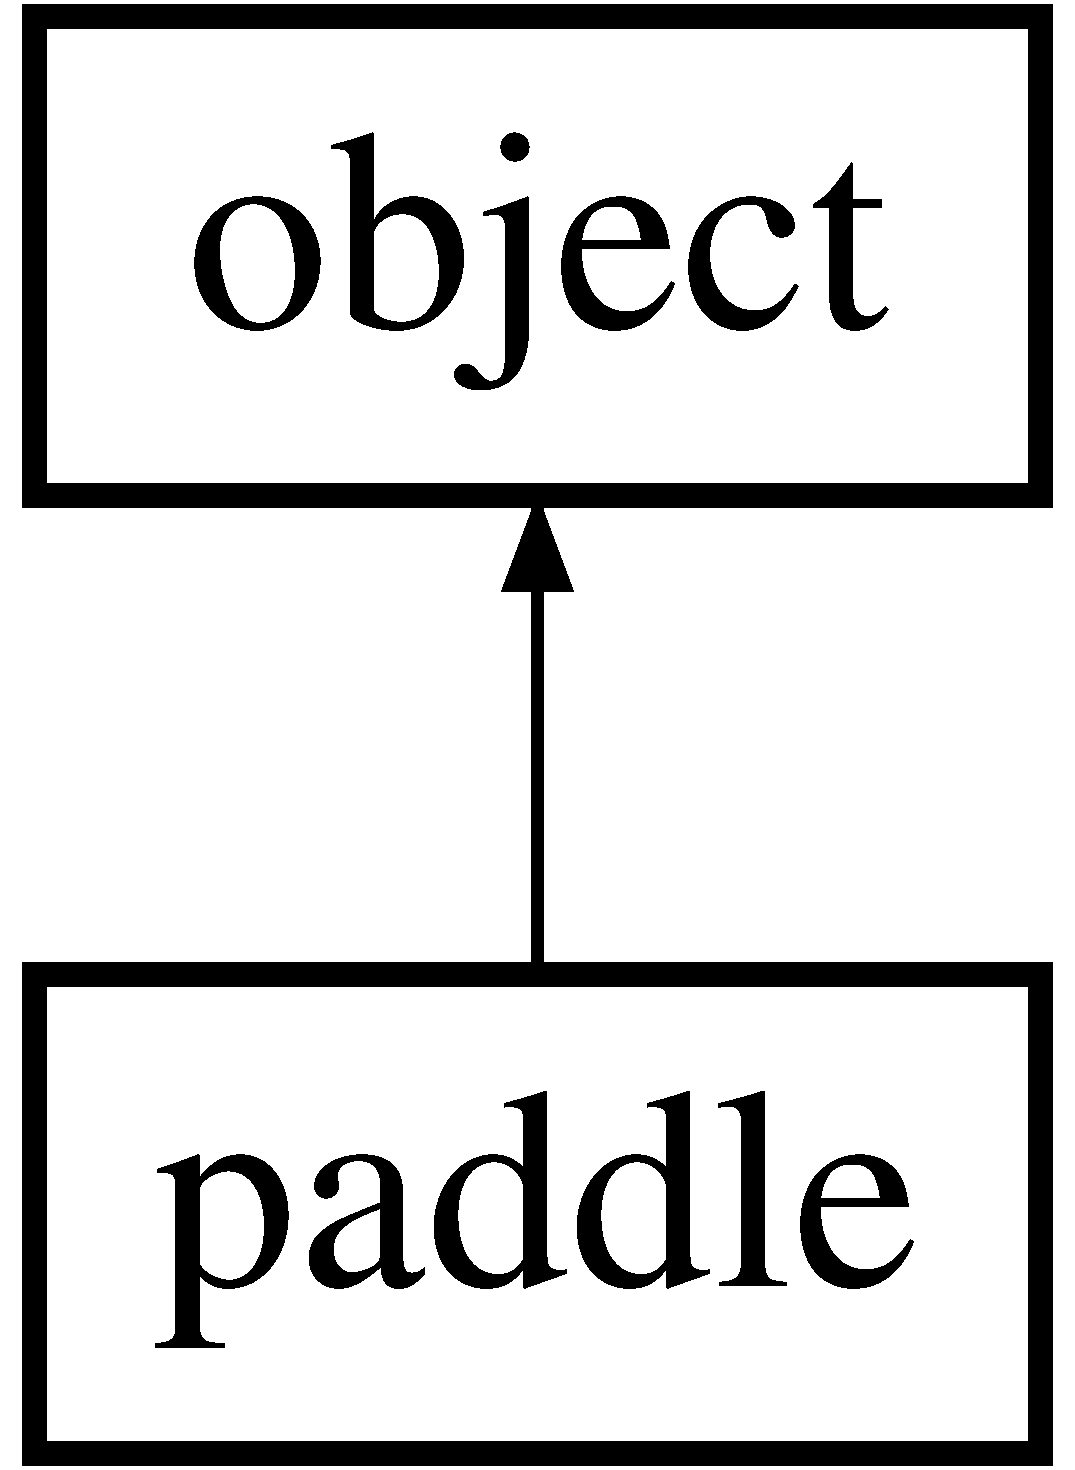
\includegraphics[height=2.000000cm]{classpaddle}
\end{center}
\end{figure}
\subsection*{Public Member Functions}
\begin{DoxyCompactItemize}
\item 
\hyperlink{classpaddle_a49204236762e7810824271d3c7c793c5}{paddle} (b2\+World \&i\+World, float i\+X\+Pos, float i\+Y\+Pos, double i\+S\+C\+A\+LE, int i\+Player)
\begin{DoxyCompactList}\small\item\em Paddle constructor. \end{DoxyCompactList}\item 
void \hyperlink{classpaddle_ae20fb7dc01d0a3b92ebc49e5d132aee8}{update} ()
\begin{DoxyCompactList}\small\item\em Update function that maintains pong speed. \end{DoxyCompactList}\item 
void \hyperlink{classpaddle_ac20b5583e5d21b34dd831f0289aae244}{handle\+Input} (sf\+::\+Event \&i\+Event)
\begin{DoxyCompactList}\small\item\em Handles paddle movement and re-\/centering. \end{DoxyCompactList}\end{DoxyCompactItemize}


\subsection{Detailed Description}
Paddle class. 

Child class of Object class for paddles used in Pong. Created by Daniel Thompson, P15230940. 

\subsection{Constructor \& Destructor Documentation}
\mbox{\Hypertarget{classpaddle_a49204236762e7810824271d3c7c793c5}\label{classpaddle_a49204236762e7810824271d3c7c793c5}} 
\index{paddle@{paddle}!paddle@{paddle}}
\index{paddle@{paddle}!paddle@{paddle}}
\subsubsection{\texorpdfstring{paddle()}{paddle()}}
{\footnotesize\ttfamily paddle\+::paddle (\begin{DoxyParamCaption}\item[{b2\+World \&}]{i\+World,  }\item[{float}]{i\+X\+Pos,  }\item[{float}]{i\+Y\+Pos,  }\item[{double}]{i\+S\+C\+A\+LE,  }\item[{int}]{i\+Player }\end{DoxyParamCaption})}



Paddle constructor. 



\subsection{Member Function Documentation}
\mbox{\Hypertarget{classpaddle_ac20b5583e5d21b34dd831f0289aae244}\label{classpaddle_ac20b5583e5d21b34dd831f0289aae244}} 
\index{paddle@{paddle}!handle\+Input@{handle\+Input}}
\index{handle\+Input@{handle\+Input}!paddle@{paddle}}
\subsubsection{\texorpdfstring{handle\+Input()}{handleInput()}}
{\footnotesize\ttfamily void paddle\+::handle\+Input (\begin{DoxyParamCaption}\item[{sf\+::\+Event \&}]{i\+Event }\end{DoxyParamCaption})}



Handles paddle movement and re-\/centering. 

\mbox{\Hypertarget{classpaddle_ae20fb7dc01d0a3b92ebc49e5d132aee8}\label{classpaddle_ae20fb7dc01d0a3b92ebc49e5d132aee8}} 
\index{paddle@{paddle}!update@{update}}
\index{update@{update}!paddle@{paddle}}
\subsubsection{\texorpdfstring{update()}{update()}}
{\footnotesize\ttfamily void paddle\+::update (\begin{DoxyParamCaption}{ }\end{DoxyParamCaption})}



Update function that maintains pong speed. 



The documentation for this class was generated from the following files\+:\begin{DoxyCompactItemize}
\item 
D\+:/\+Documents/\+Git\+Hub/\+Physics\+Game/include/\hyperlink{paddle_8h}{paddle.\+h}\item 
D\+:/\+Documents/\+Git\+Hub/\+Physics\+Game/include/\hyperlink{paddle_8cpp}{paddle.\+cpp}\end{DoxyCompactItemize}

\hypertarget{classpong}{}\section{pong Class Reference}
\label{classpong}\index{pong@{pong}}


Pong class.  




{\ttfamily \#include $<$pong.\+h$>$}

Inheritance diagram for pong\+:\begin{figure}[H]
\begin{center}
\leavevmode
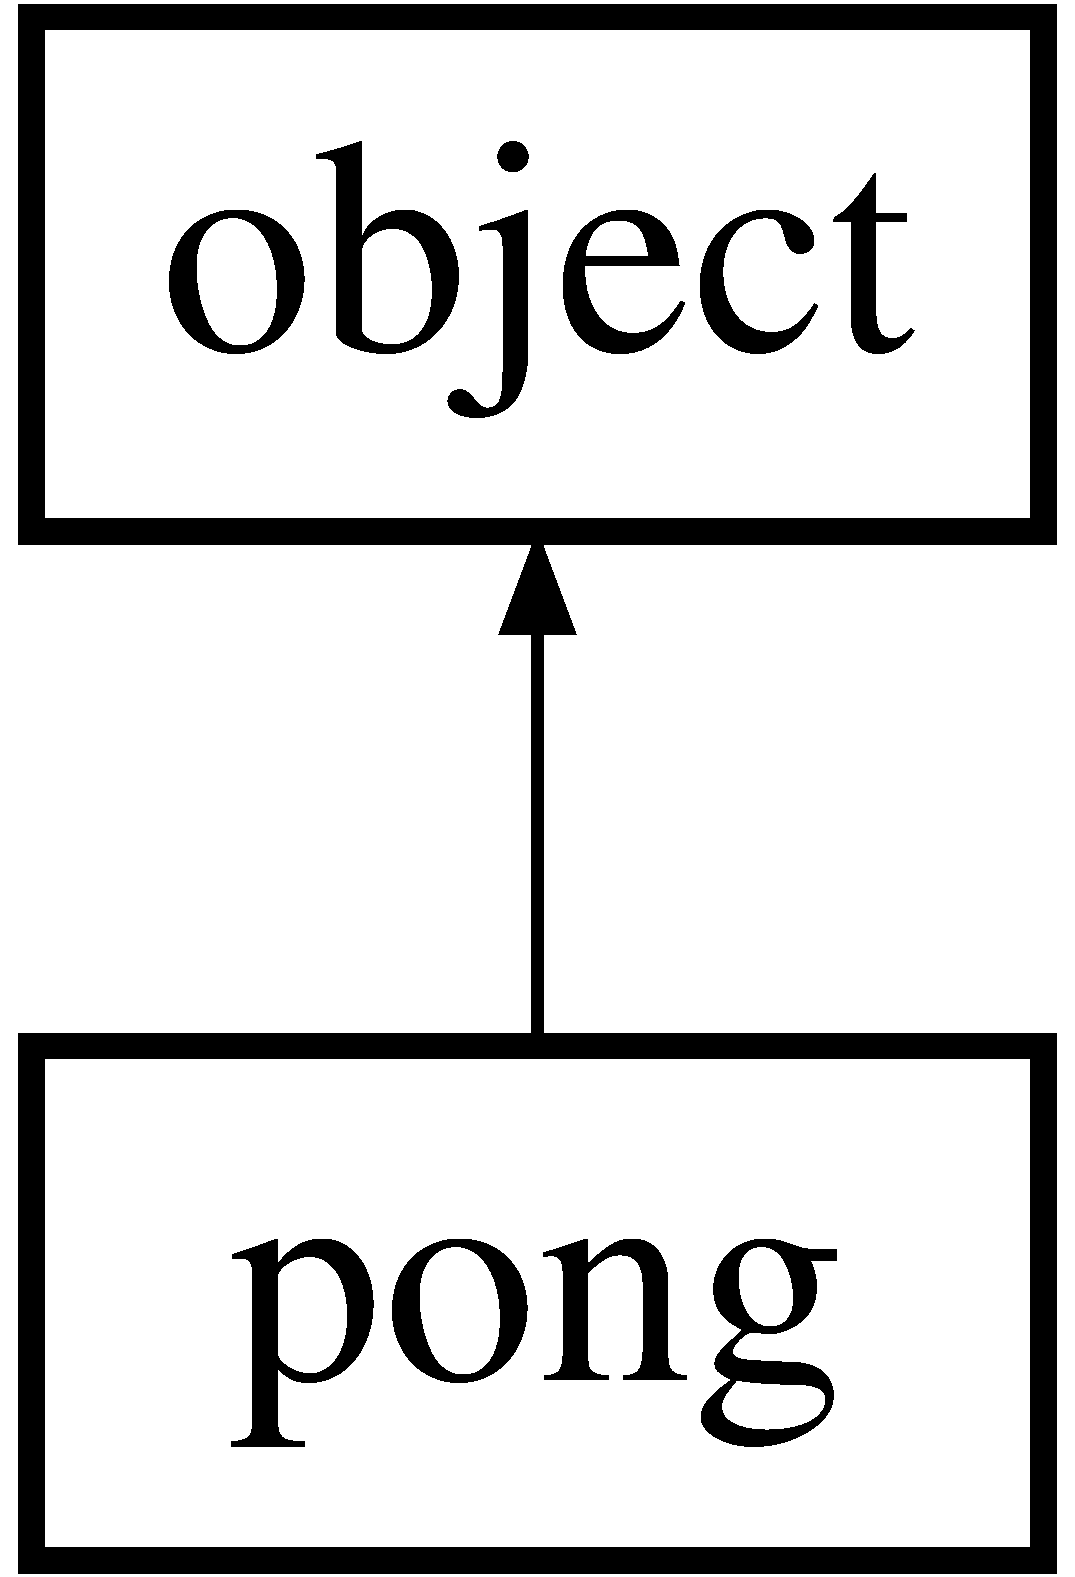
\includegraphics[height=2.000000cm]{classpong}
\end{center}
\end{figure}
\subsection*{Public Member Functions}
\begin{DoxyCompactItemize}
\item 
\hyperlink{classpong_aba99737cd7a044d2d943501433229702}{pong} (b2\+World \&i\+World, float i\+X\+Pos, float i\+Y\+Pos, double i\+S\+C\+A\+LE)
\begin{DoxyCompactList}\small\item\em Pong constructor. \end{DoxyCompactList}\item 
void \hyperlink{classpong_af5da04e472da35472a1ad0229e36480a}{start\+Moving} ()
\begin{DoxyCompactList}\small\item\em Stars pong movement. \end{DoxyCompactList}\item 
void \hyperlink{classpong_a2f36425bd4f142cf23efb4928a49f183}{update} ()
\begin{DoxyCompactList}\small\item\em Updates pong movement and increases velocity if below a threshold. Ensures pong does not stop moving horizontally. \end{DoxyCompactList}\item 
void \hyperlink{classpong_a9b9d00c224e64244a82b4c2bcea0633b}{move} (b2\+Vec2 \&i\+Velocity)
\begin{DoxyCompactList}\small\item\em Moves pong by velocity. \end{DoxyCompactList}\end{DoxyCompactItemize}


\subsection{Detailed Description}
Pong class. 

\hyperlink{pong_8h}{pong.\+h}

Child class of Object class for the pong ball used in Pong. Created by Daniel Thompson, P15230940. 

\subsection{Constructor \& Destructor Documentation}
\mbox{\Hypertarget{classpong_aba99737cd7a044d2d943501433229702}\label{classpong_aba99737cd7a044d2d943501433229702}} 
\index{pong@{pong}!pong@{pong}}
\index{pong@{pong}!pong@{pong}}
\subsubsection{\texorpdfstring{pong()}{pong()}}
{\footnotesize\ttfamily pong\+::pong (\begin{DoxyParamCaption}\item[{b2\+World \&}]{i\+World,  }\item[{float}]{i\+X\+Pos,  }\item[{float}]{i\+Y\+Pos,  }\item[{double}]{i\+S\+C\+A\+LE }\end{DoxyParamCaption})}



Pong constructor. 



\subsection{Member Function Documentation}
\mbox{\Hypertarget{classpong_a9b9d00c224e64244a82b4c2bcea0633b}\label{classpong_a9b9d00c224e64244a82b4c2bcea0633b}} 
\index{pong@{pong}!move@{move}}
\index{move@{move}!pong@{pong}}
\subsubsection{\texorpdfstring{move()}{move()}}
{\footnotesize\ttfamily void pong\+::move (\begin{DoxyParamCaption}\item[{b2\+Vec2 \&}]{i\+Velocity }\end{DoxyParamCaption})}



Moves pong by velocity. 

\mbox{\Hypertarget{classpong_af5da04e472da35472a1ad0229e36480a}\label{classpong_af5da04e472da35472a1ad0229e36480a}} 
\index{pong@{pong}!start\+Moving@{start\+Moving}}
\index{start\+Moving@{start\+Moving}!pong@{pong}}
\subsubsection{\texorpdfstring{start\+Moving()}{startMoving()}}
{\footnotesize\ttfamily void pong\+::start\+Moving (\begin{DoxyParamCaption}{ }\end{DoxyParamCaption})}



Stars pong movement. 

\mbox{\Hypertarget{classpong_a2f36425bd4f142cf23efb4928a49f183}\label{classpong_a2f36425bd4f142cf23efb4928a49f183}} 
\index{pong@{pong}!update@{update}}
\index{update@{update}!pong@{pong}}
\subsubsection{\texorpdfstring{update()}{update()}}
{\footnotesize\ttfamily void pong\+::update (\begin{DoxyParamCaption}{ }\end{DoxyParamCaption})}



Updates pong movement and increases velocity if below a threshold. Ensures pong does not stop moving horizontally. 



The documentation for this class was generated from the following files\+:\begin{DoxyCompactItemize}
\item 
D\+:/\+Documents/\+Git\+Hub/\+Physics\+Game/include/\hyperlink{pong_8h}{pong.\+h}\item 
D\+:/\+Documents/\+Git\+Hub/\+Physics\+Game/include/\hyperlink{pong_8cpp}{pong.\+cpp}\end{DoxyCompactItemize}

\chapter{File Documentation}
\hypertarget{game_8cpp}{}\section{D\+:/\+Documents/\+Git\+Hub/\+Physics\+Game/include/game.cpp File Reference}
\label{game_8cpp}\index{D\+:/\+Documents/\+Git\+Hub/\+Physics\+Game/include/game.\+cpp@{D\+:/\+Documents/\+Git\+Hub/\+Physics\+Game/include/game.\+cpp}}
{\ttfamily \#include $<$Box2\+D\textbackslash{}\+Box2\+D.\+h$>$}\newline
{\ttfamily \#include $<$game.\+h$>$}\newline
{\ttfamily \#include $<$paddle.\+h$>$}\newline
{\ttfamily \#include $<$pong.\+h$>$}\newline
{\ttfamily \#include $<$object.\+h$>$}\newline

\hypertarget{game_8h}{}\section{D\+:/\+Documents/\+Git\+Hub/\+Physics\+Game/include/game.h File Reference}
\label{game_8h}\index{D\+:/\+Documents/\+Git\+Hub/\+Physics\+Game/include/game.\+h@{D\+:/\+Documents/\+Git\+Hub/\+Physics\+Game/include/game.\+h}}
{\ttfamily \#include $<$Box2\+D\textbackslash{}\+Box2\+D.\+h$>$}\newline
{\ttfamily \#include $<$object.\+h$>$}\newline
{\ttfamily \#include $<$paddle.\+h$>$}\newline
{\ttfamily \#include $<$pong.\+h$>$}\newline
\subsection*{Classes}
\begin{DoxyCompactItemize}
\item 
class \hyperlink{classgame}{game}
\begin{DoxyCompactList}\small\item\em Game class. \end{DoxyCompactList}\end{DoxyCompactItemize}

\hypertarget{object_8cpp}{}\section{D\+:/\+Documents/\+Git\+Hub/\+Physics\+Game/include/object.cpp File Reference}
\label{object_8cpp}\index{D\+:/\+Documents/\+Git\+Hub/\+Physics\+Game/include/object.\+cpp@{D\+:/\+Documents/\+Git\+Hub/\+Physics\+Game/include/object.\+cpp}}
{\ttfamily \#include $<$object.\+h$>$}\newline

\hypertarget{object_8h}{}\section{D\+:/\+Documents/\+Git\+Hub/\+Physics\+Game/include/object.h File Reference}
\label{object_8h}\index{D\+:/\+Documents/\+Git\+Hub/\+Physics\+Game/include/object.\+h@{D\+:/\+Documents/\+Git\+Hub/\+Physics\+Game/include/object.\+h}}
{\ttfamily \#include $<$S\+F\+M\+L\textbackslash{}\+Graphics.\+hpp$>$}\newline
{\ttfamily \#include $<$Box2\+D\textbackslash{}\+Box2\+D.\+h$>$}\newline
\subsection*{Classes}
\begin{DoxyCompactItemize}
\item 
class \hyperlink{classobject}{object}
\begin{DoxyCompactList}\small\item\em Object class. \end{DoxyCompactList}\end{DoxyCompactItemize}

\hypertarget{paddle_8cpp}{}\section{D\+:/\+Documents/\+Git\+Hub/\+Physics\+Game/include/paddle.cpp File Reference}
\label{paddle_8cpp}\index{D\+:/\+Documents/\+Git\+Hub/\+Physics\+Game/include/paddle.\+cpp@{D\+:/\+Documents/\+Git\+Hub/\+Physics\+Game/include/paddle.\+cpp}}
{\ttfamily \#include \char`\"{}paddle.\+h\char`\"{}}\newline

\hypertarget{paddle_8h}{}\section{D\+:/\+Documents/\+Git\+Hub/\+Physics\+Game/include/paddle.h File Reference}
\label{paddle_8h}\index{D\+:/\+Documents/\+Git\+Hub/\+Physics\+Game/include/paddle.\+h@{D\+:/\+Documents/\+Git\+Hub/\+Physics\+Game/include/paddle.\+h}}
{\ttfamily \#include $<$object.\+h$>$}\newline
\subsection*{Classes}
\begin{DoxyCompactItemize}
\item 
class \hyperlink{classpaddle}{paddle}
\begin{DoxyCompactList}\small\item\em Paddle class. \end{DoxyCompactList}\end{DoxyCompactItemize}

\hypertarget{pong_8cpp}{}\section{D\+:/\+Documents/\+Git\+Hub/\+Physics\+Game/include/pong.cpp File Reference}
\label{pong_8cpp}\index{D\+:/\+Documents/\+Git\+Hub/\+Physics\+Game/include/pong.\+cpp@{D\+:/\+Documents/\+Git\+Hub/\+Physics\+Game/include/pong.\+cpp}}
{\ttfamily \#include \char`\"{}pong.\+h\char`\"{}}\newline

\hypertarget{pong_8h}{}\section{D\+:/\+Documents/\+Git\+Hub/\+Physics\+Game/include/pong.h File Reference}
\label{pong_8h}\index{D\+:/\+Documents/\+Git\+Hub/\+Physics\+Game/include/pong.\+h@{D\+:/\+Documents/\+Git\+Hub/\+Physics\+Game/include/pong.\+h}}
{\ttfamily \#include $<$object.\+h$>$}\newline
\subsection*{Classes}
\begin{DoxyCompactItemize}
\item 
class \hyperlink{classpong}{pong}
\begin{DoxyCompactList}\small\item\em Pong class. \end{DoxyCompactList}\end{DoxyCompactItemize}

\hypertarget{main_8cpp}{}\section{D\+:/\+Documents/\+Git\+Hub/\+Physics\+Game/\+Physics\+Game/main.cpp File Reference}
\label{main_8cpp}\index{D\+:/\+Documents/\+Git\+Hub/\+Physics\+Game/\+Physics\+Game/main.\+cpp@{D\+:/\+Documents/\+Git\+Hub/\+Physics\+Game/\+Physics\+Game/main.\+cpp}}
{\ttfamily \#include $<$S\+F\+M\+L\textbackslash{}\+Graphics.\+hpp$>$}\newline
{\ttfamily \#include $<$Box2\+D\textbackslash{}\+Box2\+D.\+h$>$}\newline
{\ttfamily \#include $<$game.\+h$>$}\newline
{\ttfamily \#include $<$object.\+h$>$}\newline
{\ttfamily \#include $<$vector$>$}\newline
\subsection*{Functions}
\begin{DoxyCompactItemize}
\item 
int \hyperlink{main_8cpp_ae66f6b31b5ad750f1fe042a706a4e3d4}{main} ()
\end{DoxyCompactItemize}


\subsection{Function Documentation}
\mbox{\Hypertarget{main_8cpp_ae66f6b31b5ad750f1fe042a706a4e3d4}\label{main_8cpp_ae66f6b31b5ad750f1fe042a706a4e3d4}} 
\index{main.\+cpp@{main.\+cpp}!main@{main}}
\index{main@{main}!main.\+cpp@{main.\+cpp}}
\subsubsection{\texorpdfstring{main()}{main()}}
{\footnotesize\ttfamily int main (\begin{DoxyParamCaption}{ }\end{DoxyParamCaption})}


%--- End generated contents ---

% Index
\backmatter
\newpage
\phantomsection
\clearemptydoublepage
\addcontentsline{toc}{chapter}{Index}
\printindex

\end{document}
